\section{Projektplanung}
\begin{figure}[H]
	\centering
	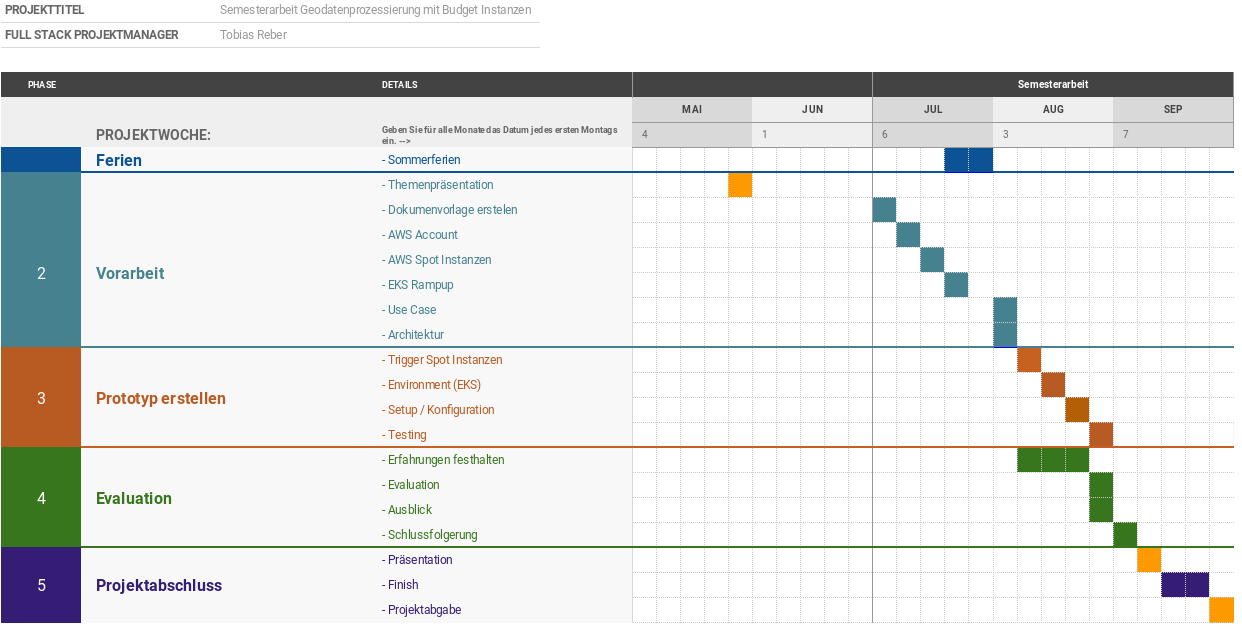
\includegraphics[width=.95\textwidth]{projektplanung}
	\caption{Projektplan}
	\label{fig:Projektplan}
\end{figure}

\section{Kennenlernen von AWS}

\subsection{EFS auf EC2-Instanz mounten}
Anhand einer Anleitung, einem sogenannten Walktrough wurde via AWS CLI (AWS Command Line Interface, einem Komandozeilenorientierten Werkzeug) ein
EFS an eine EC2-Instanz gemountet und die 3D Daten wurden dorthin kopiert.
\appendCode{bash}{EFS auf EC2-Instanz mounten}{src/walktrough_ec2_and_efs.sh}

\section{Für die Semesterarbeit verwendete Sofware}
\begin{itemize}
\item JabRef: Verwaltung des Literaturverzeichnisses
\item Gummi: Latex Editor
\item AWS CLI: Für das Bereitstellen der AWS Infrastruktur
\item jq: Für das Filtern von JSON (vor allem von AWS CLI Antworten)
\item git: Versionsmanagement der Textdateien
\end{itemize}